\documentclass[conference]{IEEEtran}
\IEEEoverridecommandlockouts
% The preceding line is only needed to identify funding in the first footnote. If that is unneeded, please comment it out.
\usepackage{cite}
\usepackage{amsmath,amssymb,amsfonts}
\usepackage{algorithmic}
\usepackage{graphicx}
\usepackage{textcomp}
\usepackage{xcolor}
\def\BibTeX{{\rm B\kern-.05em{\sc i\kern-.025em b}\kern-.08em
		T\kern-.1667em\lower.7ex\hbox{E}\kern-.125emX}}
\begin{document}
	
	\title{Report 1}
	
	\author{\IEEEauthorblockN{1\textsuperscript{st} Ali Ramezanzadeh}
		\IEEEauthorblockA{\textit{dept. of Electrical Engineering} \\
			\textit{Amirkabir University of Technology}\\
			Tehran, Iran\\
			ali.ramezan@aut.ac.ir}
		\and
		\IEEEauthorblockN{2\textsuperscript{nd} Arian Abdollahi}
		\IEEEauthorblockA{\textit{dept. of Electrical Engineering} \\
			\textit{Amirkabir University of Technology}\\
			Tehran, Iran\\
			arian.abdollahi@aut.ac.ir}
		\and
		\IEEEauthorblockN{3\textsuperscript{rd} Sina Shah Mohammadi}
		\IEEEauthorblockA{\textit{dept. of Electrical Engineering} \\
			\textit{Amirkabir University of Technology}\\
			Tehran, Iran\\
			alisinashahmohammadi@aut.ac.ir}}
	
	\maketitle

	
	\section{Introduction}
In this experiment, we want to design a lead and lag controller for an flexible joint robot.\newline
A flexible joint robot is a type of robot designed with joints that offer some degree of flexibility, compliance, or elasticity, distinguishing them from rigid robots. These robots incorporate elements like springs, elastic actuators, or specially designed mechanisms to allow controlled movement with some give or deformation at the joints. 

	\begin{figure}[htbp]
	\centerline{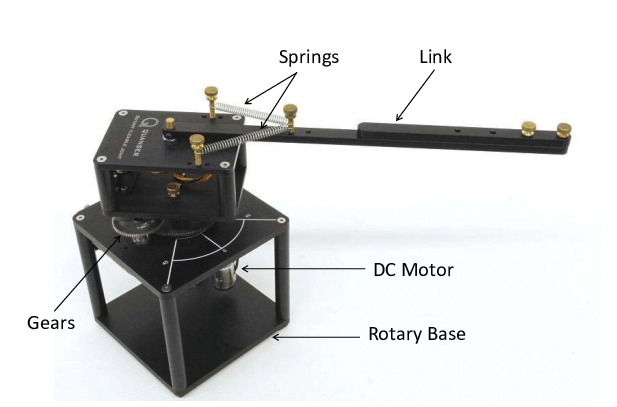
\includegraphics[width=0.7\linewidth]{1.jpg}}
	\caption{Flexible Joint Robot}
	\label{fig1}
\end{figure}

	\section{Mathematical Modeling}
We use the following diagram to derive the mathematical model of the system:

\begin{figure}[htbp]
	\centerline{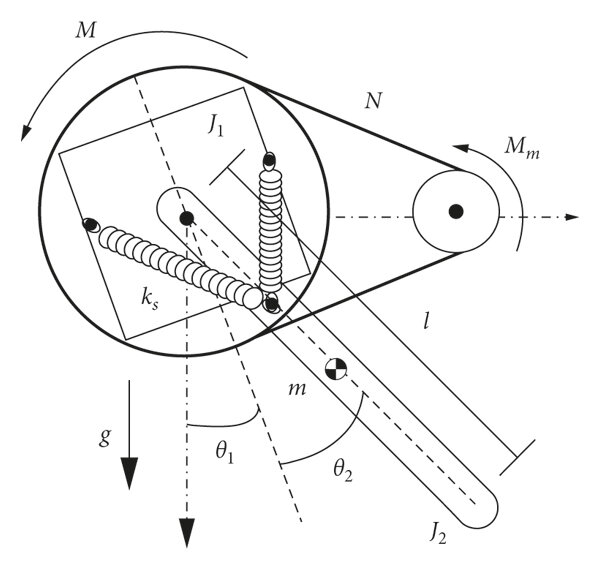
\includegraphics[width=0.7\linewidth]{2.jpg}}
	\caption{Flexible Joint Robot Model}
	\label{fig1}
\end{figure}

Using Lagrange-Hamilton, we arrive at the following equations.


\begin{equation}
	J_{eq} \ddot{\theta}+ J_{Arm}( \ddot{\theta}+\ddot{\alpha})=T_{output}-B_{eq}\dot{\theta}
\end{equation}


\begin{equation}
J_{Arm}( \ddot{\theta}+\ddot{\alpha})+K_{stiff}\alpha=0
\end{equation}

And we have the torque of a DC motor:

\begin{equation}
	T_{output}=\dfrac{\eta_{m}\eta_{g}K_{g}K_{m}(V_{m}-K_{g}K_{m}\dot{\theta})}{R_{m}}
\end{equation}
The selected state variables are:

\[
X=
\begin{pmatrix}
	\theta \\
	\dot{\theta}\\
	\alpha \\
	\dot{\alpha}\\
\end{pmatrix}
\]


Then, using the solve command in MATLAB, we solve the above equations and obtain the state-space matrices:

\[
A=
\begin{pmatrix}
	0 & 1 & 0 & 0 \\
	0 & {\frac{- (K_m  K_t  n_g  n_m   K_g^2 + B_{eq}  R_m)}{a}} & {\frac{K_{stiff}}{J_{eq}}} & 0 \\
	0 & 0 & 0 & 1 \\
	g &  {\frac{ (K_m  K_t  n_g  n_m   K_g^2 + B_{eq}  R_m)}{a}} & {\frac{-K_{stiff}(J_{arm}+J_{eq})}{J_{eq}J_{arm}}} & 0 \\
\end{pmatrix}
\]

\[
B=
\begin{pmatrix}
	0 \\
	\dfrac{K_{t}K_{g}\eta_{g}\eta_{m}}{J_{eq}R_{m}} \\
	0 \\
	-\dfrac{K_{t}K_{g}\eta_{g}\eta_{m}}{J_{eq}R_{m}} \\
\end{pmatrix}
\]

\[
C=
\begin{pmatrix}
	1 & 0&0 &0  \\
\end{pmatrix}
\qquad D=0
\]


\section{Calculations for design Lead-Lag controller }
\begin{equation}
	K_{v} = 50     
\end{equation}
\begin{equation}
	\phi_{des} = 80^\circ
\end{equation}
\begin{equation}
	\omega_{g} = 5
\end{equation}


To design a lead-lag controller, we first need to obtain the steady-state error coefficient K :
\begin{equation}
	K_x = \lim_{s \to 0} s^N \cdot G(s)
\end{equation}
\begin{equation}
	K = 28.408 
\end{equation}
Now multiply K in our transfer function and then we find the phase margin from our Bode diagram , and then find the $\phi_{m}$ from Equation 9.
\begin{equation}
	\phi_{m} = \phi_{P.M.d} - \phi_{P.M} + \Delta 
\end{equation}
With $\phi_{m}$ and the given frequency, we can calculate $\alpha_{lead}$ .With this information, we find the zero and pole of the lead:
\begin{equation}
	\sin(\phi_{m}) = \frac{\alpha_{lead} - 1}{\alpha_{lead} + 1} 
\end{equation}
\begin{equation}
	\alpha_{lead} = \frac{P_{lead}}{Z_{lead}} 
\end{equation}
\begin{equation}
	\omega = \sqrt{p \times z} 
\end{equation}
\begin{equation}
	Z_{lead} = -4.08  ,  P_{lead} = -6.12  
\end{equation}
Then, to design lag, we place the zero at one-tenth of the frequency w and, using Equation 15, we find the $\alpha_{lag}$ and pole of the lag :
\begin{equation}
	Z_{lag} = -0.5 
\end{equation}
\begin{equation}
	20\log(\alpha_{lag}) + 10\log(\alpha_{lead}) = -\lvert GH_{(jw)} \rvert
\end{equation}
\begin{equation}
	\alpha_{lag} = 0.1 , P_{lag} = -0.05
\end{equation}
At the end, equation 17 represents the final controller :
\begin{equation}
	G_{c} = K \times \alpha_{lag} \times \alpha_{lead} * \left( \frac{s + z_{lag}}{\alpha s + p_{lag}} \right) * \left( \frac{s + z_{lead}}{\alpha s + p_{lead}} \right)
\end{equation}
After add controller to system we see that the controller satisfied the given conditions :

\begin{figure}[htbp]
	\centerline{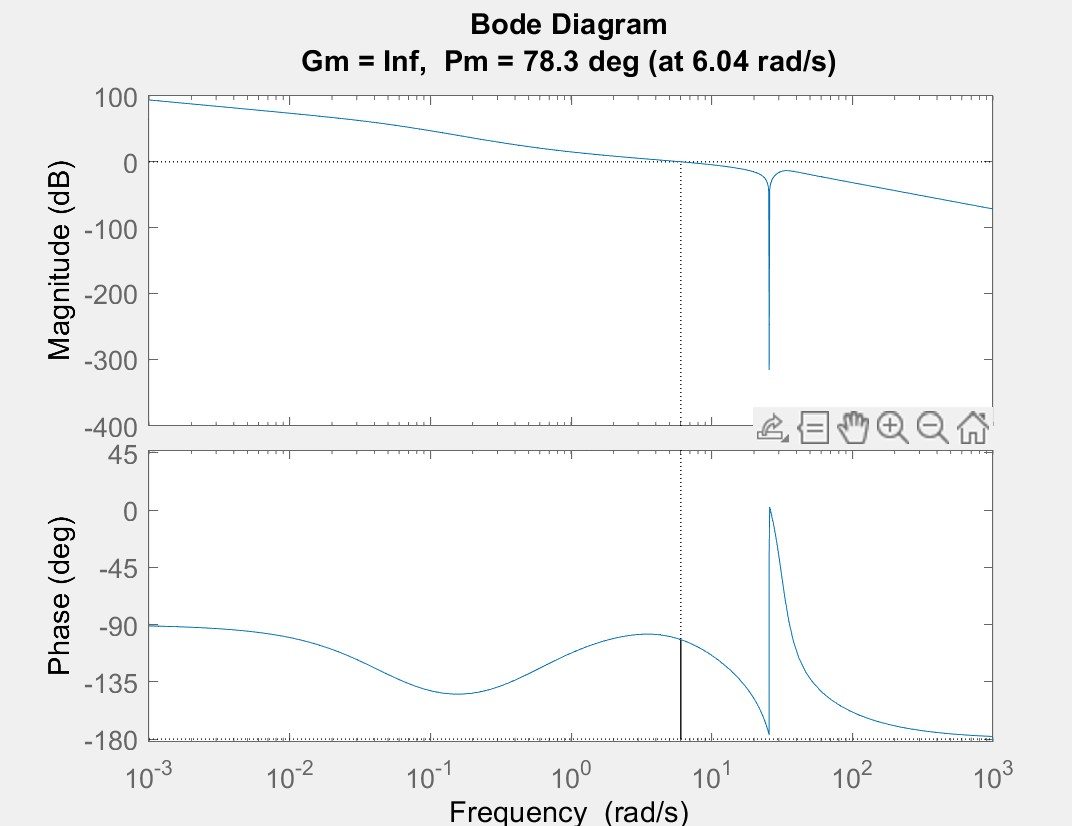
\includegraphics[width=0.9\linewidth]{3.jpg}}
	\caption{Bode with controller}
	\label{fig3}
\end{figure}
\newpage
This is our step response after add controller :
\begin{figure}[htbp]
	\centerline{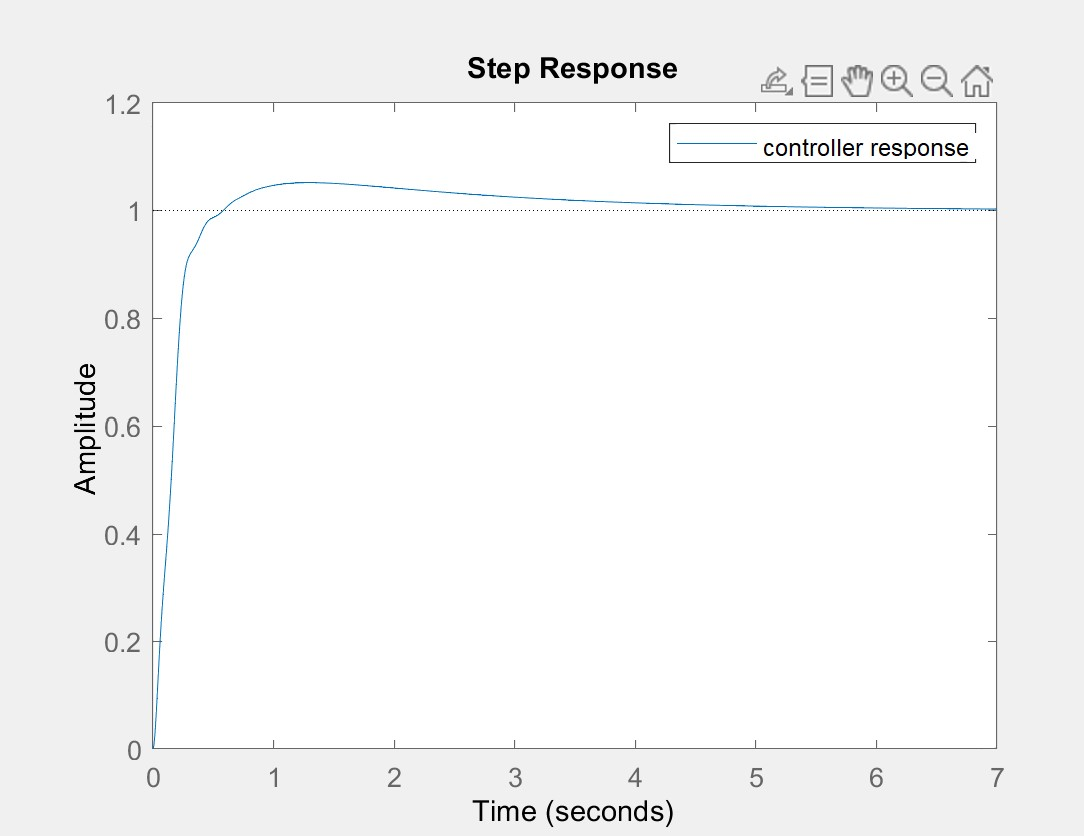
\includegraphics[width=0.9\linewidth]{4.jpg}}
	\caption{Step response}
	\label{fig4}
\end{figure}

Now we test our system on flexible joint robot and see the results :

\begin{figure}[htbp]
	\centerline{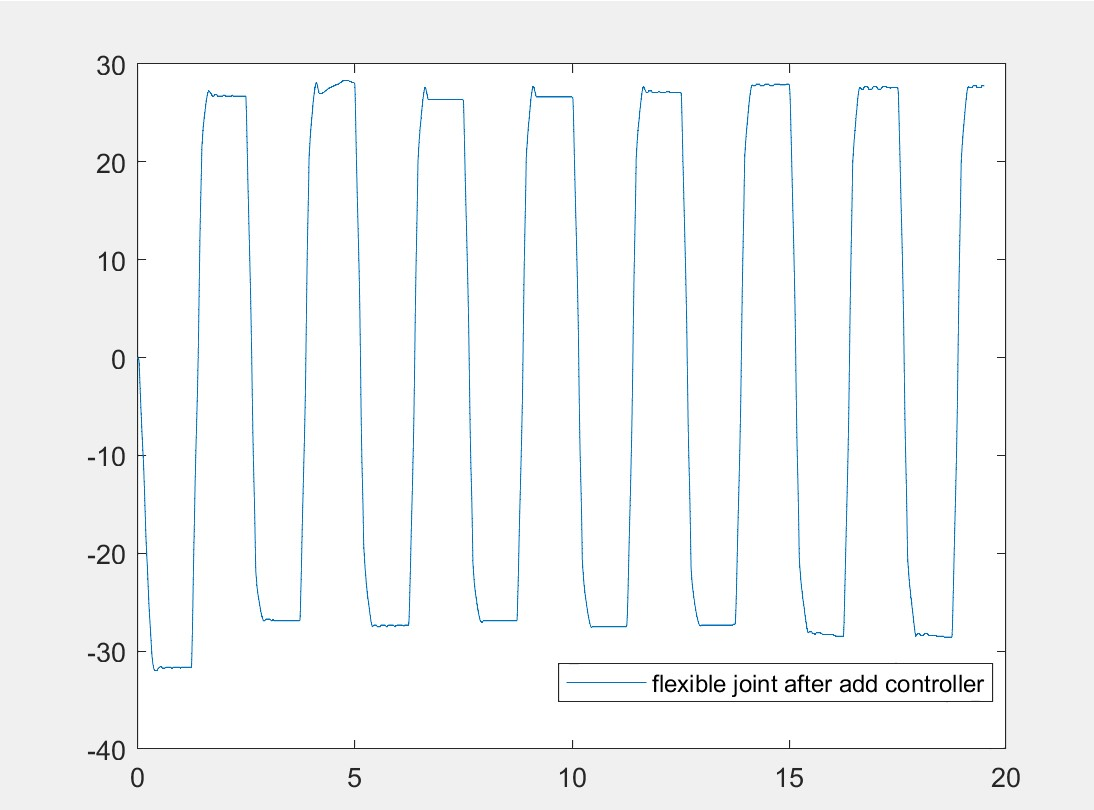
\includegraphics[width=0.9\linewidth]{5.jpg}}
	\caption{flexible joint response after add controller}
	\label{fig5}
\end{figure}

as we see, the controller was able to both increase the speed of the system and reduced the error.
\end{document}

